\chapter{The visual display of structured population dynamics and STdiag its implementation in R}\label{Chap:STDiag}
\chaptermark{Structure-time diagrams}
\vspace{4cm}

\begin{Spacing}{1}
\texttt{
Le Bourlot, Vincent, François Mallard, Caroline Ligier, Manuel Massot, 
David Claessen, and Thomas Tully, "The visual display of structured population dynamics and STdiag its implementation in R".\\
under review at Ecology and Evolution
}
Voir Chapitre \ref{chap:method} Section \ref{sec:stdiag}.
\end{Spacing}

\section*{Abstract}
\addcontentsline{toc}{section}{Abstract}

%\begin{enumerate}
  %\item 
  
\lettrine[lines=3]{I}{n demography}, a detailed study of the temporal dynamics
of a population structure is often required to better understand the processes
that underline the overall dynamics and the individual life histories.

Heatmaps using time and structure (such as size-structure) as x and y
coordinates and density as colors are efficient tools for displaying the
dynamics of a structured population. Such representations (structure-time
diagrams), reveal the data at several levels, from general outlook to fine
details.

This graphical display is a simple and efficient way to make large demographic
datasets coherent and to disclose the underlying often hidden demographical
processes. But despite its efficiency, this method has been scarcely used in
ecology and demography.

To emphasise how rich this graphical representation is and to illustrate that
this method can be applied even outside the field of ecology, we present several
case studies: a long-term survey of different collembolan populations in a
laboratory microcosm, a 16 year survey of a wild common lizard population, the
daily consumption of antibiotics in France during one year and the dynamics of
the age-structure of the French population during the last century.

We present the R package \texttt{STdiag}, an interface to complex graphical
functions to easily produce and analyse such "structure-time diagrams" from raw datasets.
This package is available for all operating systems via R-Forge. Its syntax and
options are described, discussed and illustrated using our case studies.
% \end{enumerate}

\section{Introduction}

Structured populations are complex assemblages of individuals differing in age,
size or body condition, reproductive stage or physiological state (Fig.
\ref{fig:ASTd1}a, b).
The dynamics of structured populations are often complex, hard to follow and
difficult to understand and analyse \autocites{benton2006a}.
Depending on their state, size, and age, the individuals have different
demographic performances and respond differently to demographic parameters
(competition, interactions) or environmental factors (such as resource,
temperature).
Furthermore, population structures are shaped by the complex interplay of both
biotic and abiotic effects \autocites{ohlberger2013a}.
For an individual, the effect of the demographic feedback loop depends on the
state of the individual itself but also on the structure of its population. For
instance, if large individuals dominate the smaller ones through interference
competition in a population, the strength of the competition perceived by an
individual is determined in a complex manner by its own body size and by the
size-structure of the population (Chapitres \ref{chap:sp},\ref{chap:amnat},
\ref{chap:sm}, Annexe \ref{An:AmNat}). The demographic responses to
environmental change can also be non trivial because the sensitivity of the
individual’s demographic performances to an environmental effect may differ
depending on the state, age or size of the individuals
\autocites{ohlberger2011a}.
A gradual change in temperature can for example suddenly destabilise the
population dynamics which can shift abruptly towards a new regime
\autocites{ohlberger2011a, nelson2013a}. This complexity is increased again by
the fact that the dynamics of a structured population is influenced not only by
the current biotic and abiotic conditions but also by long term effects due to
long lasting effects of previous environmental conditions
\autocites{baron2010a,mugabo2010a} and to inter-generational effects
\autocites{benton2008a,marquis2008a}.

Given the multiple causes that influence population dynamics and the complexity
of the direct and indirect mechanisms through which they drive the population
dynamics, we argue that extracting relevant biological information from
structured population time series requires not only to fit complex demographic
models to the data, but also to study graphs of the population structure
dynamics which can themselves contribute to understanding what happens in the
population. When used on their own, models and calculations can be misleading
since they rely on assumptions that may be false. But good graphical display can
reveal, without distorting, what the data have to say
\autocites{tufte2001a}.
Graphs can be very valuable for studying the data at several levels of detail, to look for
signatures of past conditions on the dynamics, to verify the validity of the
model’s assumptions and even to suggest alternative ways of setting up the
statistical analysis \autocites{anscombe1973a}. The aim of this paper is
to present a simple graphical method for displaying the temporal dynamics of structured
populations which can be used to visualise large and complex demographic
time-series efficiently, revealing the details and nuances of the complex
demographic processes that occur in most populations. We argue that such
graphical displays are essential tools for ferreting out the devils hidden in
the details of structured population dynamics \autocites{benton2006a}.

\begin{figure}[!ht] % Figure 1 
\centering
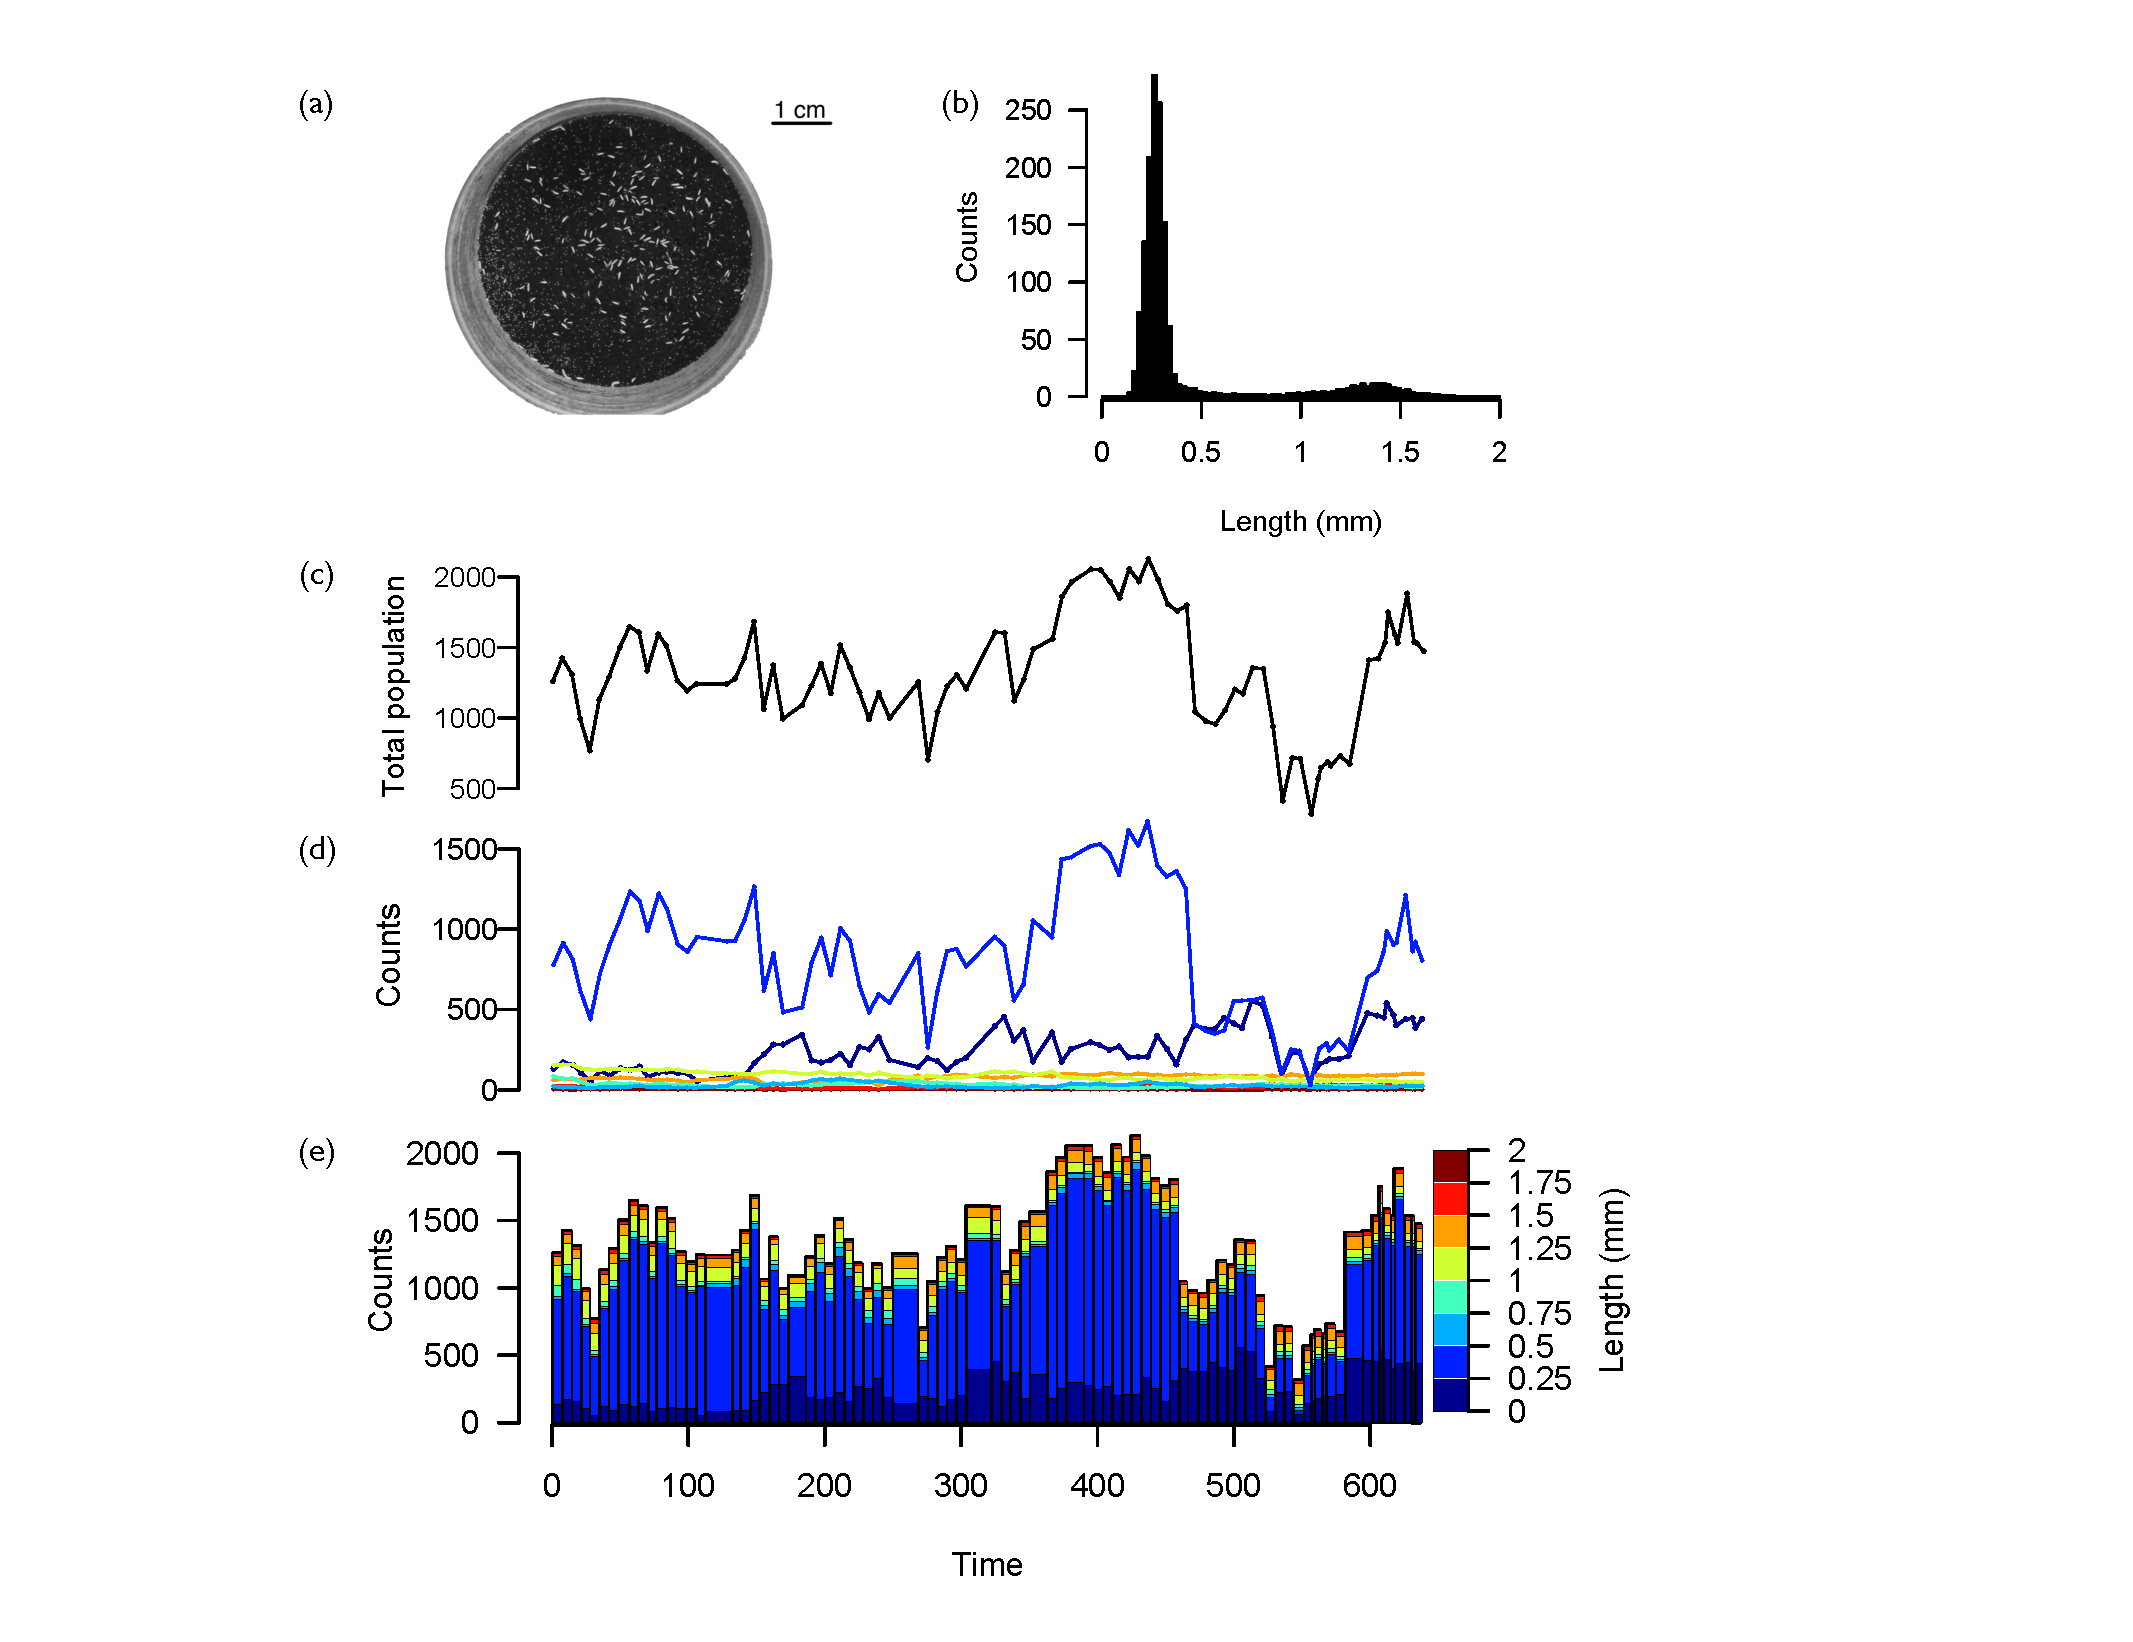
\includegraphics[height=0.75\textheight]{2_Methodo/Fig/01}
\caption[\lofimage{2_Methodo/Fig/01}Classical representation of a population
structure]{We used as a practical example an experimental population of the
Collembola \textit{Folsomia candida} (a) whose structure has been measured every
one or two weeks. The size structure at one time is classically shown as a histogram
(b) and the total population dynamics on a time series plot (c). To represent
both the structure and temporal dynamics, the population has been divided in
several size classes to plot their dynamics independently (d) or to produce a
stacked bar plot (e). While these representations underline the dynamics inside
each size classes, the patterns of dynamics between adjacent classes remain
hidden.
}
\label{fig:ASTd1}
\end{figure}


Different approaches have been used to display structured population dynamics
(Fig. \ref{fig:ASTd1}c, d, e): by displaying the whole population size
fluctuations, the structure is not taken into account (Fig.  \ref{fig:ASTd1}c)
\autocites{schrautzer2011a}. The structure can be roughly considered by
splitting individuals into separate groups (of size or stages) whose dynamics
can be displayed on adjacent plots \autocites{plaistow2009a} or, to facilitate
comparisons, on overlaid curves (Fig.
 \ref{fig:ASTd1}d) or on a stacked bar plot (Fig.  \ref{fig:ASTd1}e)
 \autocites{madsen2000a}. But condensed three-dimensional diagrams are required
 to finely display the structure dynamic especially when the structuring factor
 is continuous (size, age). These diagrams
encompass “event history diagrams” that allow the graphical representation of
life history traits at the individual level of a whole cohort
\autocites{carey1998a,carey2008a} or the production of “shaded contour maps”
such as the ones used to represent the temporal dynamics of aged-structured
demographic rates like death or birth rates in human populations
\autocites{vaupel1997a,vaupel1998a}. These graphical representations are mainly
used in human demography to represent secular changes in age-dependent
demographic rates
\autocites{vaupel1987a,vaupel1997a,vaupel1998a,andreev2000a,erlangsen2003a}. To
our knowledge, despite their interest, such powerful visual displays have almost
never been used in ecology to represent the temporal dynamics of structured
populations \autocites{faerovig2002a}. This may result
from the prohibiting cost of publishing colour pictures. But with the development of
online publishing, colour methods are becoming more widely used. The R software
\autocites{team2012a} is a language and
environment for data manipulation, calculation, statistical computing and graphic display. Heatmaps
can be produced using base packages (e.g. image in graphics and heatmap in
stats) or using specific libraries such as lattice
\autocites{sarkar2008a} or ggplot2 \autocites{wickham2009a}. But although
highly customizable, the plotting functions are often difficult to handle for beginners.

We made the R-package STdiag to provide a user-friendly interface for
representing time series of structured populations using heatmaps. We detail how
to generate such graphics and discuss their biological interests using (i) the
long-term structure dynamics of experimental laboratory populations of the
Collembola Folsomia candida, (ii) a long-term study of a
population of common lizards Zootoca vivipara in France, (iii) an example
in the field of pharmaco-epidemiology -- the seasonal dynamics of the annual
consumption of antibiotics in France -- and (iv) the temporal dynamic
of the age by sex structure of the French population during the last century.

\section{Method overview}

Our method produces diagrams that we refer to as "structure-time diagrams", with
a structuring element (age, size,\ldots) along the Y-axis and time along the
X-axis. These variables are usually continuous but are discretised in a
histogram and put into several classes, the number and width of which depend on
the quality and size of the available dataset. For each time and structure class
coordinate, a colour rectangle is plotted whose hue refers to the number of
individuals (or any other statistics such as frequency or rate) in that class
(possibly on a logarithmic scale) at the given time. This representation puts
side-by-side colour histograms for each time value and emphasises the temporal
dynamics according to the structure of the population.

\section{Package STdiag usage}

To easily display the dynamics of a structured population we made the package
STdiag, which is freely available at R-forge (R-forge.r-project.org/) and can be
installed in R with the following command:

\texttt{install.packages("STdiag",repos="http://r-forge.r-project.org",type="source")}

\subsection{Importaing and formating the data}

\subsubsection{Data frame}
\texttt{STdiag} uses the \texttt{lattice} function \texttt{levelplot}
\autocites{sarkar2008a} as the core plotting function. As a consequence, the
basic data format is a three column data frame containing the $X$ (time), $Y$
(structure such as age or size) and $Z$ (number of individuals) coordinates. The
data frame has $T \times S$ lines where $T$ is the number of time values and $S$
the number of structure classes.

\subsubsection{Matrix}
Another possibility is to use a matrix description of the data using two vectors
$x$ and $y$ of size respectively $T$ and $S$ for the time and structure
coordinates, and a matrix $z$ of size $T \times S$ containing the number of
individuals at each coordinate. This mimics the format used by function image
\autocites{team2012a}. In case one wishes to
convert data from the matrix to the frame format, the function
\texttt{Matrix2DataFrame} is provided:

\texttt{DataFrame <- Matrix2DataFrame(z, x, y, xlab="time", ylab="structure",
zlab="number")}.

\subsubsection{Individual based data}
The function \texttt{Indiv2DataFrame} is also provided to convert individually
based data to a data-frame that can be plotted with \texttt{STdiag}. This
function handles a data-frame containing one line per individual, and in columns for each
individual the time of the observation and the value of the structuring element.
The option \texttt{classes}, allows to control the number of classes to
discretise the structure variable. A single value produces the wanted number of regular classes
(default set to 50), whereas a vector specifies the breaks of the classes as in
function hist. This function is used as follows:

\texttt{DataFrame <- Indiv2DataFrame(IndivData, classes=50)}

or 

\texttt{DataFrame <- Indiv2DataFrame(IndivData, classes=seq(0,10,0.1))}.

\subsection{Generating the plots}

\subsubsection{Data frame}
The simplest way to generate the basic plot is to use the data frame
formulation. If the columns of the data frame are in a time-structure-number
order, a simple call to

\texttt{STdiag(DataFrame)}

will produce the plot. If one wants to specify what column to plot, the function
STdiag accepts the formula syntax:

\texttt{STdiag(number ~ time * structure, data= DataFrame)}.

In any of those or the following forms, the vector used as time can either be a
numeric vector or a vector of dates of classes \texttt{POSIXlt},
\texttt{POSIXct} or \texttt{Date}.
Class \texttt{factor} is not yet supported for date format.

\subsubsection{Matrix}
To use the matrix formulation, call either

\texttt{STdiag(Matrix)}

in which case $X$ and $Y$-axes will be default vectors from 1 to respectively
$T$ and $S$. Or, if one wants to specify the $x$ and $y$ coordinates,

\texttt{STdiag(x=time, y=structure, z=Matrix)}.

\subsection{Improving the graphical representation}

Our method is implemented with several options to adjust the plot to be as
informative as possible.

\begin{figure}[!ht] % Figure 2 
\centering
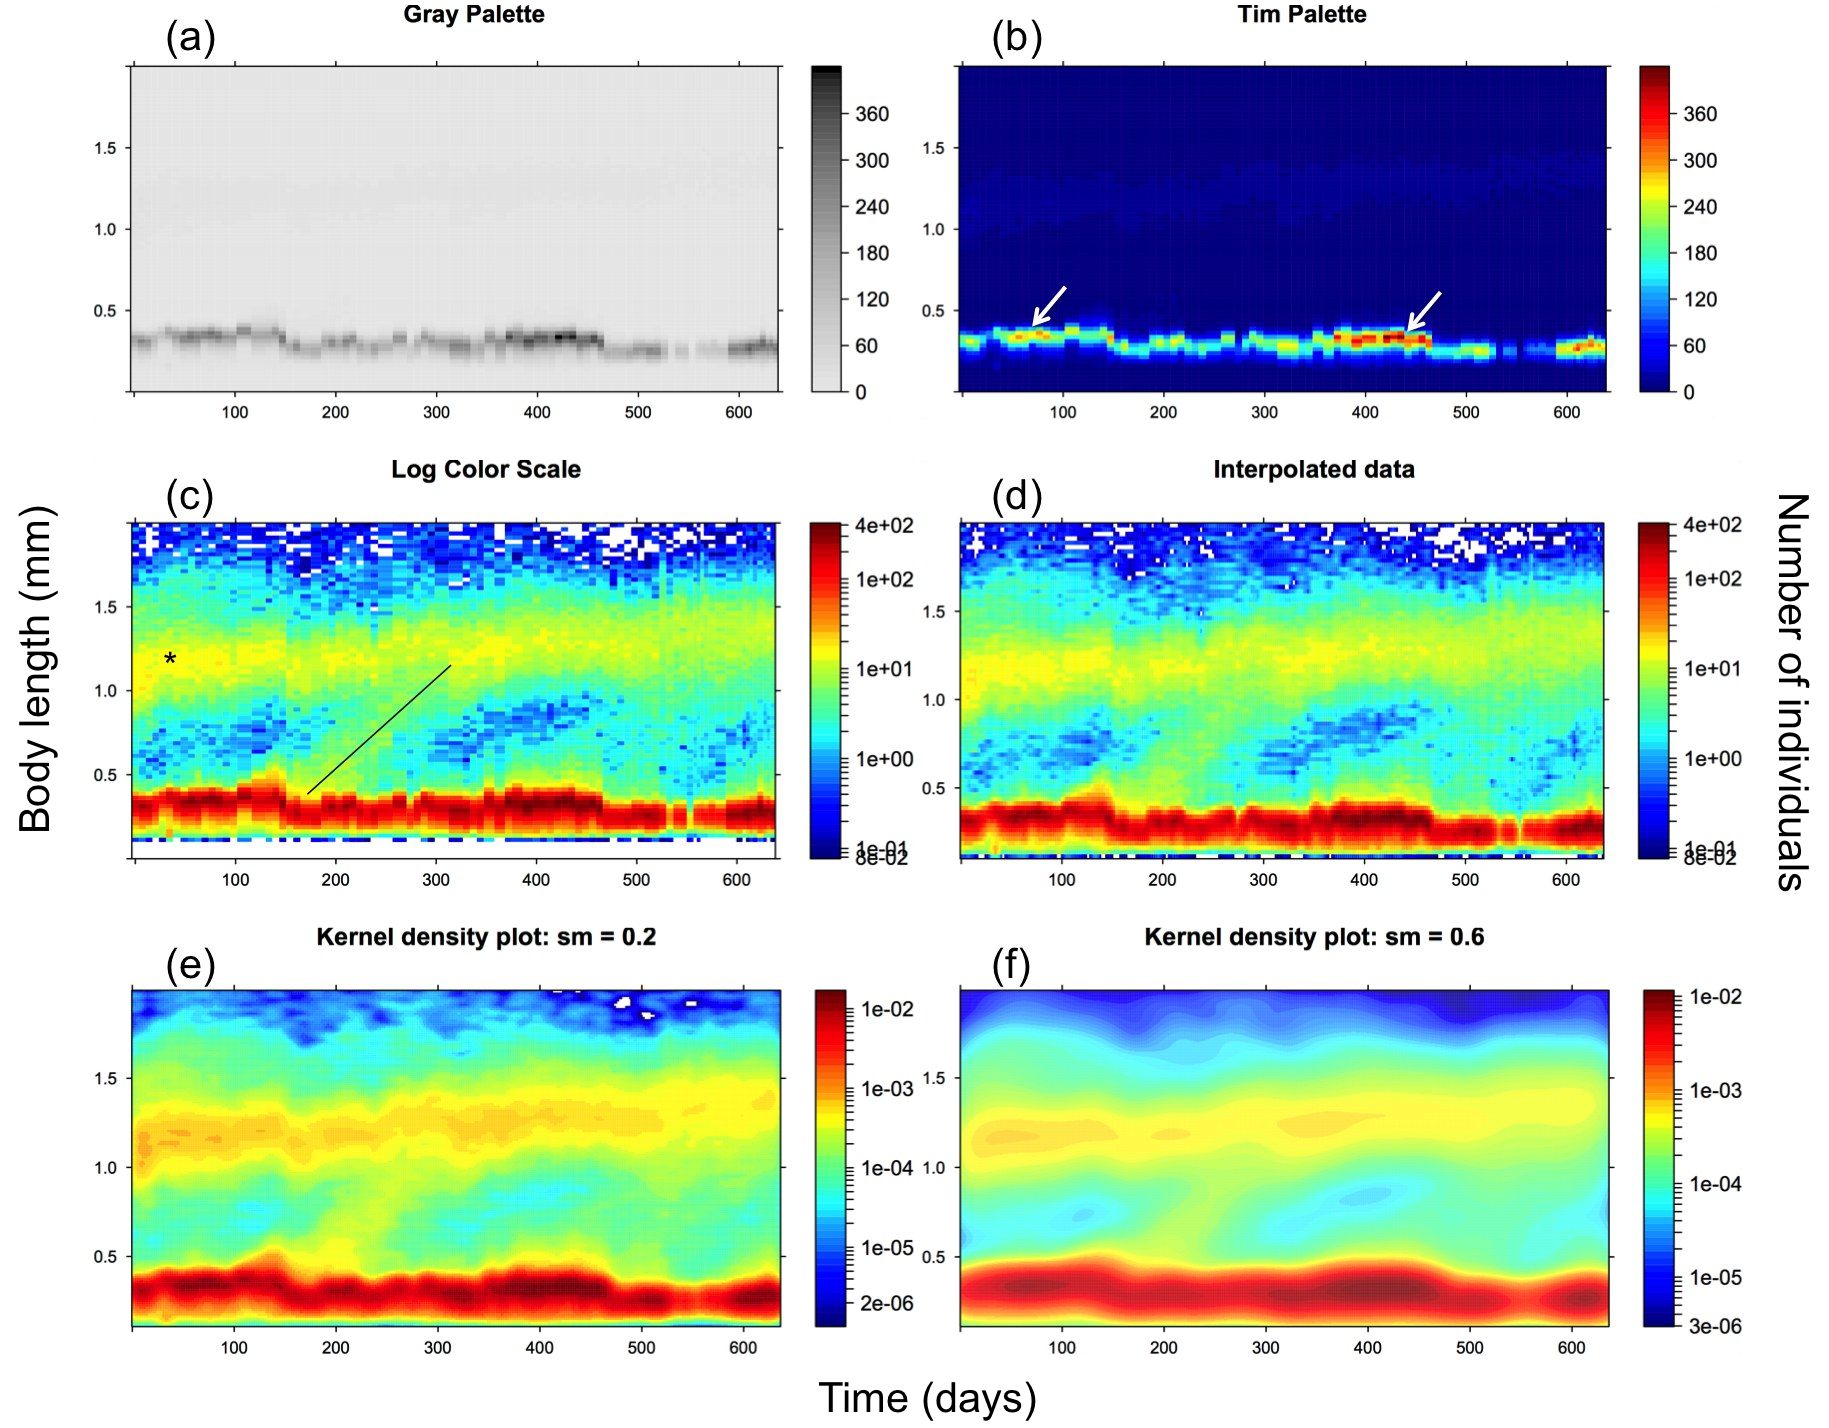
\includegraphics[width=0.95\textwidth]{2_Methodo/Fig/02}
\caption[\lofimage{2_Methodo/Fig/02}Collembolan population dynamics plotted with
STdiag]{Collembolan population dynamics plotted with \texttt{STdiag}. The code
to produce each plot is given in each panel. Length is discretised into classes
of $0.05mm$ length. Number of individual at each date length coordinate is
represented on a linear grey (a) or colour (b) scale or on a logarithmic scale (c, d). Panel (d)
represents an interpolated version of panel (c). Panels (e) and (f) represent
two kernel density estimates with increasing smoothness. The population is
mostly composed of small individuals ($\approx 0.4mm$) living with some adults
($\approx 1.2mm$).
Logarithmic scale reveals details about the recruitment of some cohorts, the
growth rate of which can be estimated (black lines, c). See Supporting
Information for details about the options used to produce the different plots.}
\label{fig:ASTd2}
\end{figure}

\subsubsection{Colour palette}
The readability of the diagram partly relies on the choice of colours for the
palette (Fig. \ref{fig:ASTd2}a, b). The hues are sorted following either a grey
scale from pale grey to black or an adapted rainbow gradient (Fig.
\ref{fig:ASTd2}a, b, c). This can be adjusted using the option
\texttt{color="palette"} inside \texttt{STdiag()} where palette can be one of
the following: gray, topo, terrain, heat, cm, rainbow or by default tim
\autocites[see tim.colors in library fields,][]{furrer2012a}.

\subsubsection{Logarithmic scale}
When the number of individuals in the different classes differs by several
orders of magnitude (Fig. \ref{fig:ASTd1}b) we recommend using a logarithmic
scale to increase the readability of the generated graphics.
The option \texttt{log=TRUE/FALSE} allows the user to switch easily between
linear and logarithmic colour scales (Fig. \ref{fig:ASTd2}c).

\subsubsection{Interpolation}
The quality of the diagram can sometimes be improved by applying an
interpolation to smooth the representation and link together uneven time
intervals by creating evenly spaced data (Fig. \ref{fig:ASTd2}d). The
interpolation method creates an artificial dataset with evenly distributed data, based on the
original data. It is essential to make a clear distinction when reading such a
diagram between the real data and data created by the interpolation and we
recommend to first use a non-interpolated representation of the data. To
interpolate the data, we provide in the package the function
\texttt{Interpolation}.
This function is an interface to function \texttt{interp.surface} in package
fields adapted to quickly handle data in the format accepted by function
\texttt{STdiag}. It takes as argument the data frame to be interpolated in the
form of three columns: time, structure and number of individuals, in that order.
The options \texttt{intervX} and \texttt{intervY} allow the user to manually
choose the intervals between two interpolated points, respectively over $X$
(time) and $Y$ (structure) axes. If those options are left empty, the function
uses the minimum distance between two points in the first and second columns as
intervals for respectively $X$ and $Y$-axes.

\subsubsection{Kernel density estimate}
The function STdiag provides an option \texttt{smooth=TRUE/FALSE} to plot a
weighted kernel density estimate of the data using an axis-aligned bivariate
normal kernel, where the data are the time-structure coordinates weighted by the
number of individuals. The estimate is derived from the function \texttt{kde2d}
in package \texttt{MASS} \autocites{venables2002a}. The density estimate can be
adjusted with options \texttt{sm}, a positive scalar (0 meaning the original
data and 1 being the normal reference distribution kernel estimation bandwidth) defining
the smoothness of the kernel density estimate, and \texttt{n}, the number of
points on the $X$ $Y$ grid. Together, these options allow  viewing a smooth
representation of the structured data (Fig. \ref{fig:ASTd2}e, f, Fig.
\ref{fig:ASTd4}).
Contrary to the interpolation, the kernel density estimate only provides a smooth representation of the data. In
the case of missing data, such as irregular time intervals, interpolating the
data before plotting the kernel density can avoid having gaps in the density for
a low smoothing factor (small \texttt{sm}).

\subsubsection{Getting some quantitative measurements from the diagrams}

The function \texttt{STdiag.measure} can be used to interact with the diagram
and get some quantitative measurement from it.

\texttt{STdiag.measure(stdiag,type=c("point","line"))} 

\texttt{stdiag} is the output from function \texttt{STdiag}. When the function
is called, it will wait for the user to identify via mouse clicks one or two
points (depending on the option \texttt{type}) in the panel being drawn. If used
with the option \texttt{type="point"}, it returns the position of the point
identified with a single mouse click. This can be useful for example when
measuring on a diagram the mean size at birth (white arrows on Fig.
\ref{fig:ASTd2}b) or the average size of a group of adults (star on Fig.
\ref{fig:ASTd2}c). If used with the option \texttt{type="line"}, one has to
click twice on the diagram and the function returns the slope of the line
defined by the two points along with the coordinates of the points. This can be
used to measure directly on the graphs the growth rate of a cohort (line on Fig.
\ref{fig:ASTd2}c), the secular change of the size of adults in a population
(Fig. \ref{fig:ASTd3}) or the linear climb of the front of ageing towards older
ages during the last century (Fig. \ref{fig:ASTd6}). Finally, the option
\texttt{region=TRUE/FALSE} provides the possibility to extract a region of the plot, i.e. a subset of the data around
the chosen point or line.
With this option, option range allows to adjust the window of selection.

\section{Reading and interpreting structure time diagrams through four case studies}
\sectionmark{Reading and interpreting ST diagrams}

\subsection{Dynamics of laboratory populations of collembolans}

We applied our graphical representation method with the help of the STdiag
package to several case studies. As a first practical example, we used some data
from the monitoring of experimental populations of Folsomia candida (Fig.
\ref{fig:ASTd1}a), a parthenogenetic springtail (see Supporting Information for
methodological details). Measures of the number and size of individuals (Fig.
\ref{fig:ASTd1}b) are taken every one or two weeks during about $600$ days
($\approx 85$ weeks) using image analysis \autocites{mallard2013a}.

\begin{figure}[!ht] % Figure 3 
\centering
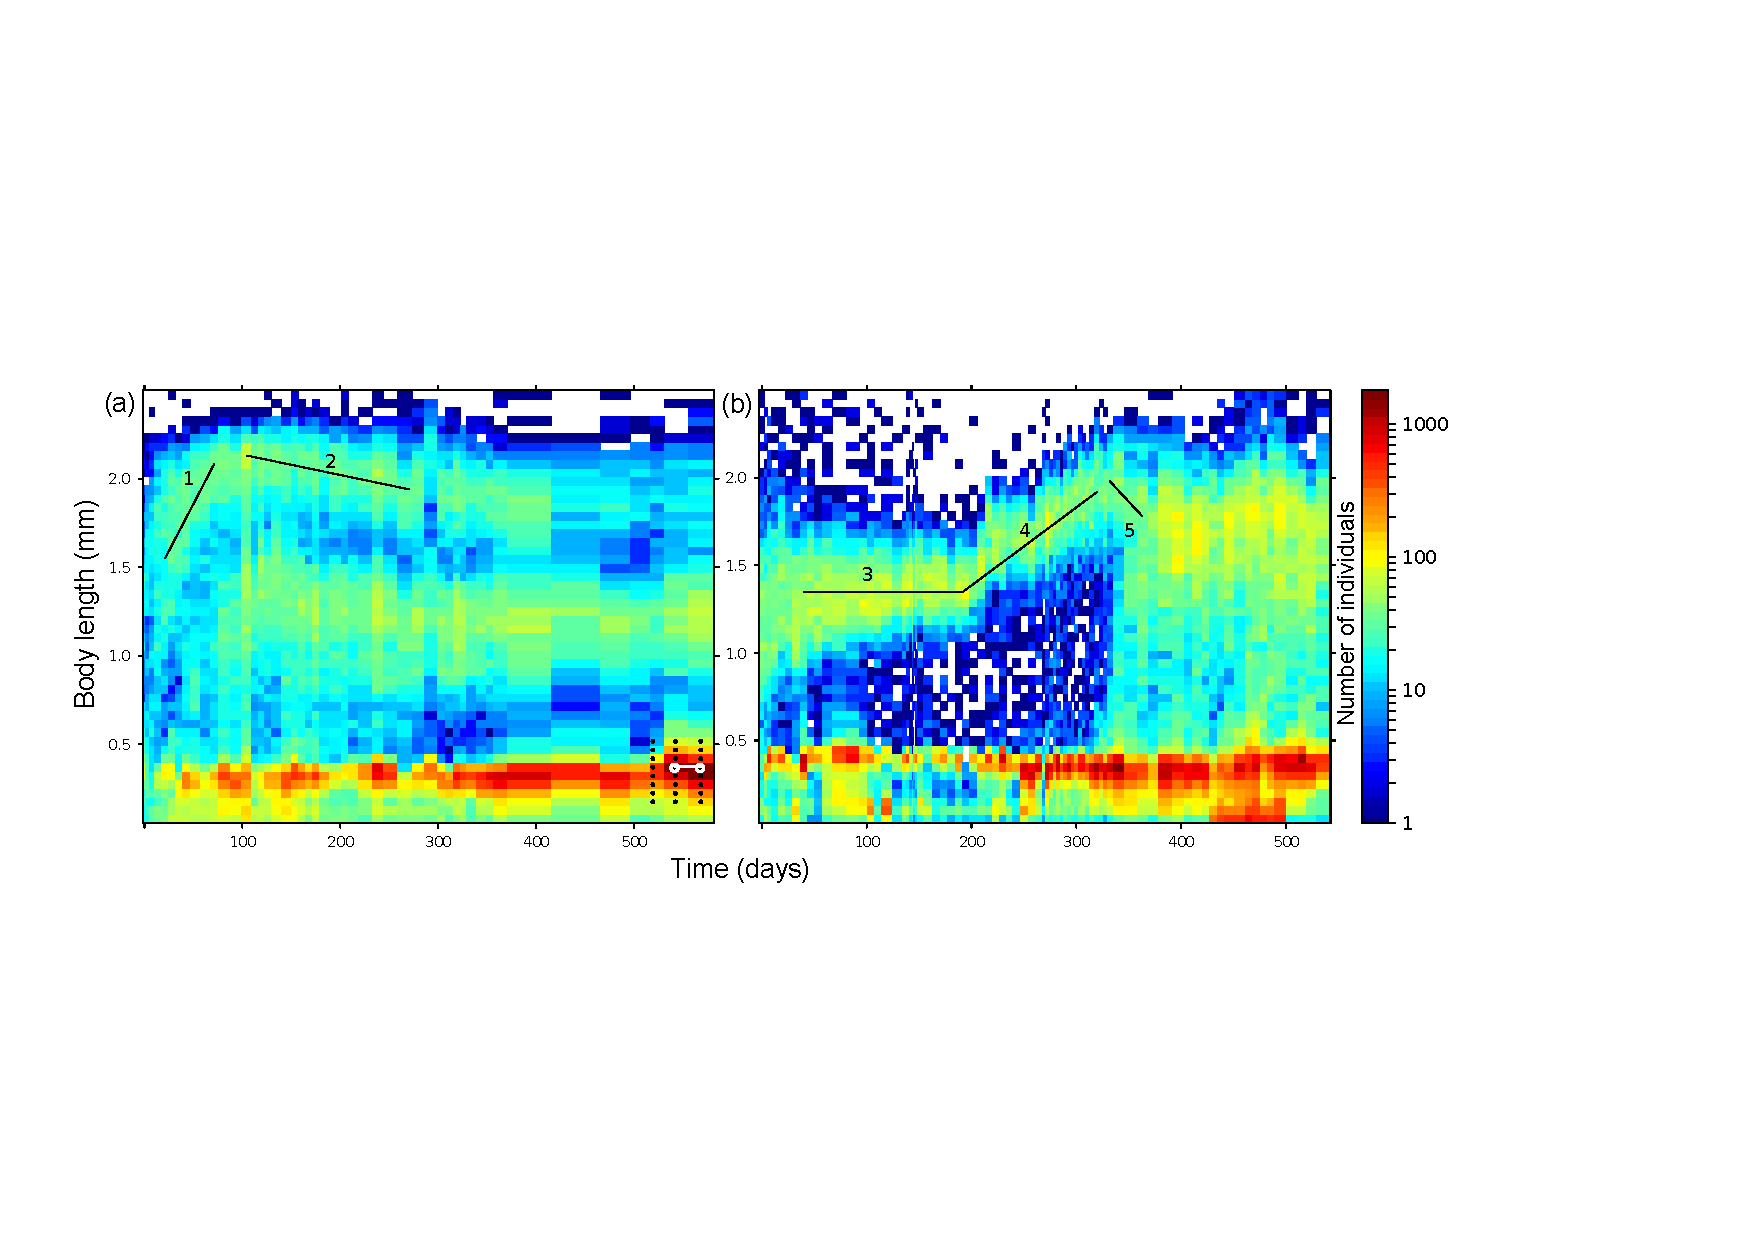
\includegraphics[width=0.95\textwidth]{2_Methodo/Fig/03}
\caption[\lofimage{2_Methodo/Fig/03}Two laboratory populations of collembolans]{
Two laboratory populations of collembolans followed during 1.6 years.
(a) Three cohorts of juveniles grow and recruit during the first 20 weeks. The
third cohort reaches a smaller adult size than the first two. After 20 weeks the
population structure reaches an almost stable trimodal distribution made of
large and small adults and of juveniles that do not manage to grow anymore. This
graphic also reveals that the mean size of the cohort of large adults shrink
between week 20 and 40 (line 2). (b) This diagram shows the remarkable
plasticity of the cohort of adults, which can resume growth after 35 weeks when
the amount of food provided has increased. But it is only after week 60, when
the adults have ceased growing that the juvenile can benefit from the improved
environmental conditions by growing themselves. These two graphs reveal the
strong size-dependent interference competition, which is a primary factors that
drive the population structure dynamics in this system.}
\label{fig:ASTd3}
\end{figure}

The structure-time diagrams (Fig. \ref{fig:ASTd2}, Fig. \ref{fig:ASTd3})
immediately reveal the predominance of the younger class (<.5mm). The populations are usually bimodal (juveniles and
adults, Fig. \ref{fig:ASTd2}, Fig. \ref{fig:ASTd3}b) and sometimes trimodal
(small and large adults; Fig.
\ref{fig:ASTd3}a). The use of a log scale (Fig. \ref{fig:ASTd2}c) reveals some
inter-class dynamics undetectable when using classical representations: for
example, between day $150$ and day $300$ a cohort of small individuals grows and
changes into adults. This visual display allows one to estimate some demographic parameters that cannot be
seen on classical representations (Fig. \ref{fig:ASTd1}) using the function
STdiag.measure described above: size at birth ($\approx 0.28mm$, by observing
spikes of births, white arrows of Fig. \ref{fig:ASTd2}b), median adult length
($1.2mm$ around day $50$, black star of Fig. \ref{fig:ASTd2}b), growth rate of a
cohort of juveniles fighting to be recruited in the population ($0.22 mm/month$,
slope of the straight line of Fig. \ref{fig:ASTd2}c). It is also possible to
study the long-term temporal dynamics of adult body length.
Depending on different conditions (intensity of competition, quantity of
resource, temperature) the mean length of the adults in the population can
remain stable (Fig. 3b, line 3), increase (Fig. \ref{fig:ASTd3}a, line1, Fig.
\ref{fig:ASTd3}b, line 4) or even decrease (Fig. \ref{fig:ASTd3}a, line 2 \&
Fig.
\ref{fig:ASTd3}b, line 5).
These graphics illustrate the remarkable plasticity of body length of the collembolans, which can plastically
adjust their body length upwards and downwards during most of their lifespan.

\subsection{Dynamics of a wild population of common lizards.}

As a second study example we used individual-based mark-recapture data collected
from 1989 to 2004 in a wild population of common lizards in southern France (see
Supporting Information for details). Fig. \ref{fig:ASTd4} clearly shows the long
term dynamic of the population structure: males are on average smaller and less captured than
females. Compared to other examples, the dynamic of the population structure is
relatively discontinuous (Fig. \ref{fig:ASTd4}). The population structure is
multimodal along the size axis because of the annual reproduction, and is discontinuous along the
time axis because the sampling was not performed during the six months of the
hibernation period. The sampled population is composed of new-borns
($\approx 2cm$), yearlings ($\approx 4cm$) and adults ($>5cm$). The figure also
shows at a glance some secular changes in the mean size of both adults and yearlings: the body length
in the population increases from 1989 to 1994
\autocites{chamaille-jammes2006a} and decreases thereafter.

\begin{figure}[!ht] % Figure 4 
\centering
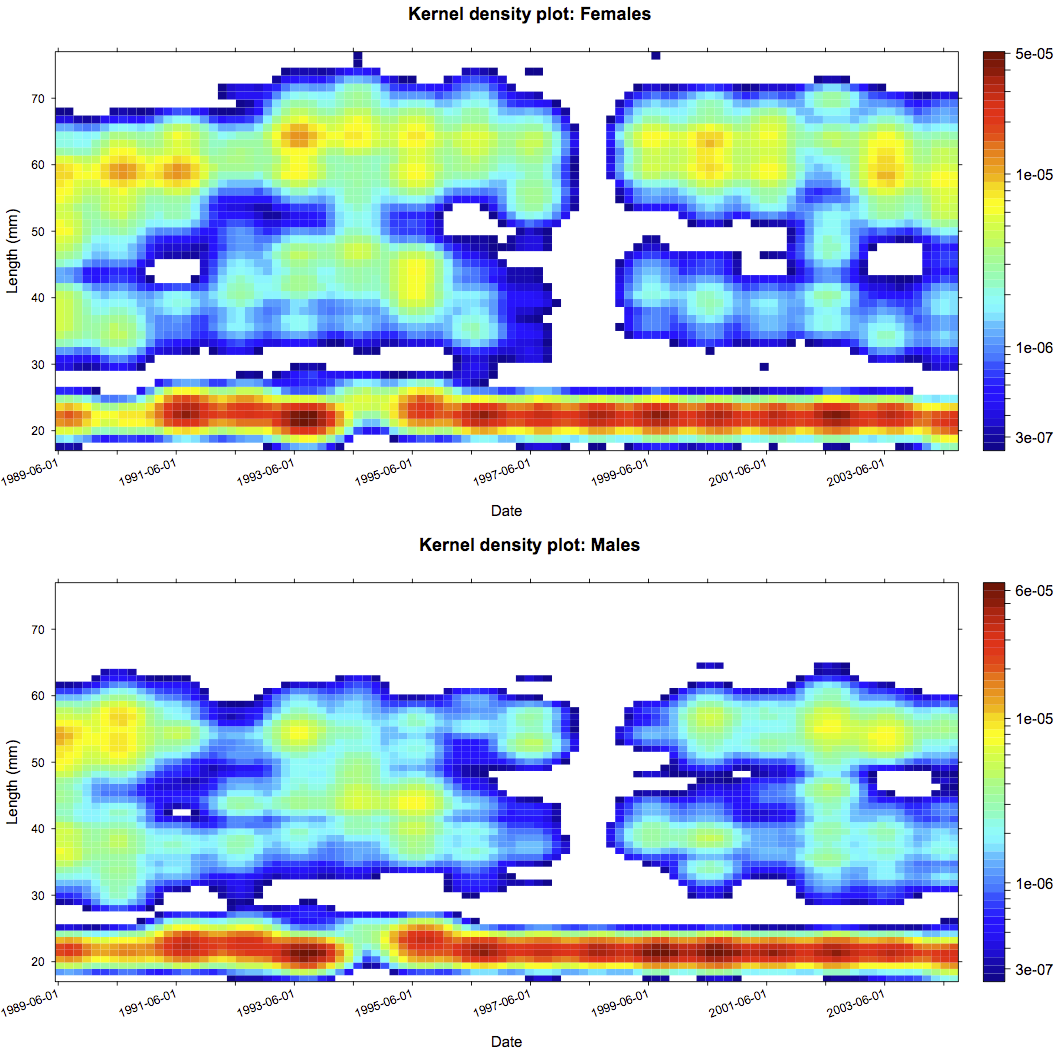
\includegraphics[width=0.95\textwidth]{2_Methodo/Fig/04}
\caption[\lofimage{2_Methodo/Fig/04}The follow-up of a population of the common
lizard]{The follow-up of a population of the common lizard. The plots represent
the population size structure (snout-vent length) of the animals - (a) females
and (b) males - captured in the population each spring. Captured pregnant
females are kept in the laboratory until parturition and the juveniles are
measured right after birth. In 1998, for exceptional reasons the prospection
effort was very low and very few adults of sub-adults have been captured and
measured. The population structure and the long-term changes of snout-vent
length can be easily seen on these graphs. We used here a log scale and a kernel
density plot. The large "dots" that are apparent with regular frequency on the
Female plot result from the seasonal annual census of the population.
}
\label{fig:ASTd4}
\end{figure}


\subsection{Antibiotics consumption during the H1N1 influenza pandemic}

Our next example - the consumption of antibiotics in France - is an application
of our method in the field of pharmaco-epidemiology. It illustrates the
efficiency of this graphical display to make database of tens of millions of
observations almost instantaneously understandable. We have used data from the
French national database provided by the CNAMTS (“Caisse nationale d’assurance
maladie des travailleurs salariés”, national fund of health insurance for
employees), which covers $75\%$ of the French population. In this specific
example, one can easily see that the purchase of antibiotics decreases every
weekend and during public holiday because most of the chemist shops are closed
(vertical bars on Fig. \ref{fig:ASTd5}a). One can see also that on average, more
antibiotics are purchased for children than for adults. But more interestingly,
the plot reveals the seasonal change in antibiotic consumption for each age
class in the population (Fig. \ref{fig:ASTd5}a): the seasonal variation in
children antibiotic consumption follows the periods of holidays while for adults
and elderly people, the plot (Fig. \ref{fig:ASTd5}a) specifically underlines the detailed
topology of the burden of purchases that has arisen during the H1N1 influenza
pandemic which occurred from September 2009 to January 2010 in France (Fig.
\ref{fig:ASTd5}b, c) \autocites{lemaitre2010a,lemaitre2012a}.

\begin{figure}[!ht] % Figure 5 
\centering
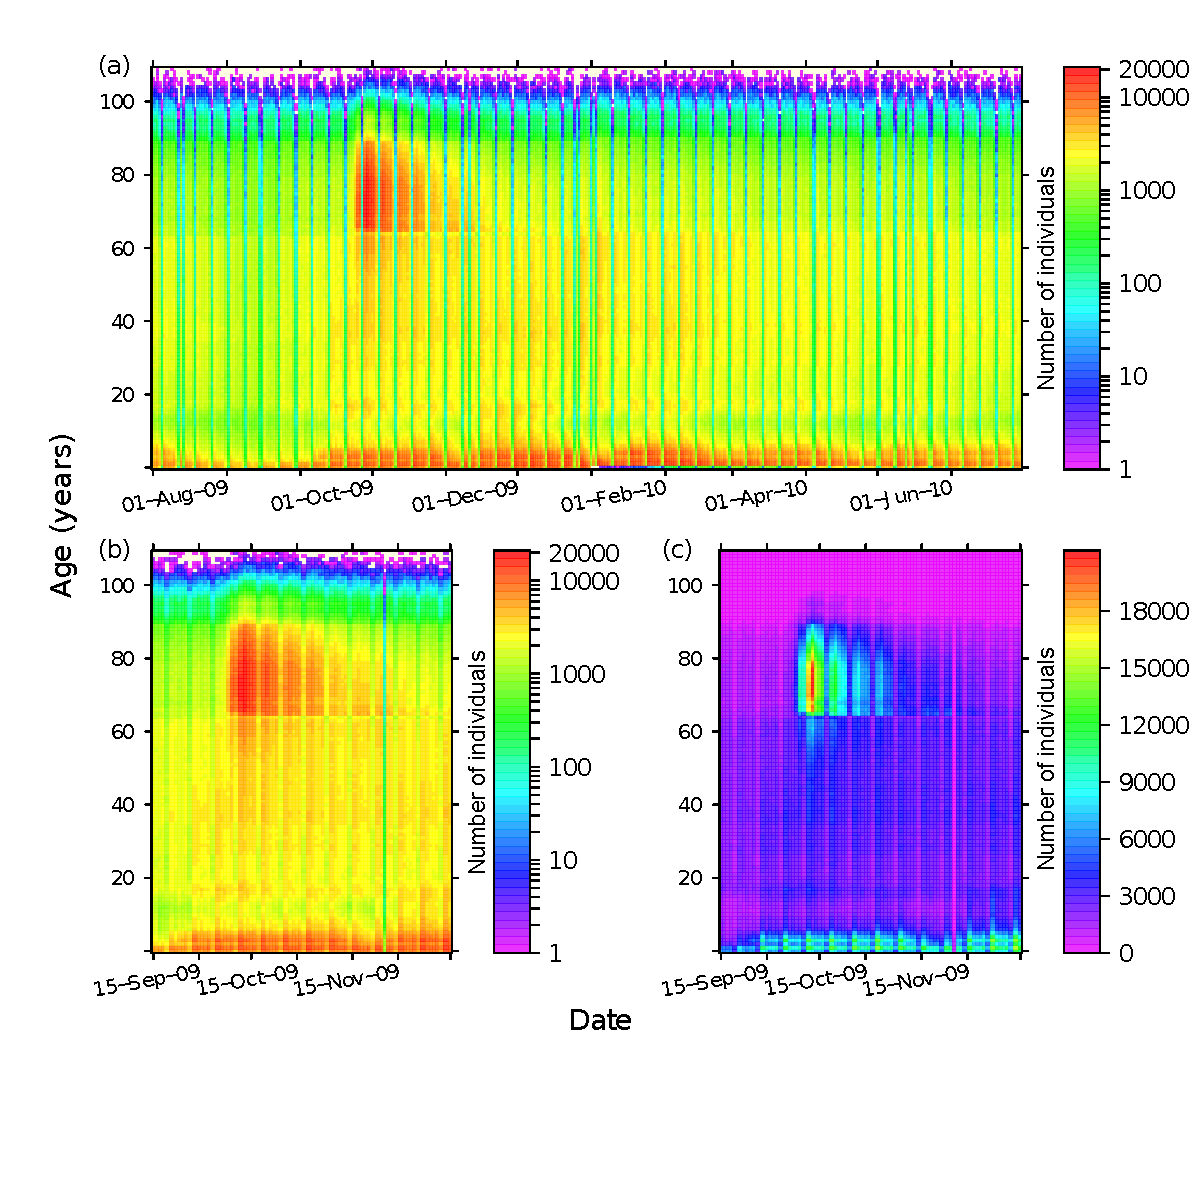
\includegraphics[width=0.9\textwidth]{2_Methodo/Fig/05}
\caption[\lofimage{2_Methodo/Fig/05}Antibiotic consumption in France]{ Graphical
representation of the antibiotic consumption in France from 1st July 2009 to
30th June 2010. The number of antibiotics bought in chemist’s shop is shown for
each age class (68 millions of observations). (a) The full representation
reveals the structure by week (the purchases of antibiotic falls off during the
weekend and public holiday), the seasonal fluctuations (less consumption during
spring and summer seasons) and a wave of consumption in autumn 2009. The
vacations give rhythm to the children’s antibiotic consumption. Removing
Saturday and Sunday allows a cleaner view of the data, and a close-up view on
the autumnal wave of purchases on a logarithmic (b) or linear (c) scale reveals
the increase in antibiotics consumption following the outburst of H1N1 during
that period. }
\label{fig:ASTd5}
\end{figure}

\subsection{The age-structure dynamics of the French population during the last
century}

Human demographers usually study human population structure by plotting age
pyramids. To illustrate the long-term temporal dynamics of human population
structure some authors use multiple age pyramids \autocites{vallin1999a}.
An ST-diagram is much more efficient since on a single pair of panels one can plot
all the whole information contained in dozens of age pyramids. We used as an
example some data based on the French population during the last century. This
data is freely available from the French national institute of statistical and
economic information \autocites{insee2010a}. We made Fig. \ref{fig:ASTd6} using
the data from 108 age pyramids. This figure represents by sex, the dynamics of the age-structure of
the French population from 1901 to 2013. It reveals many interesting parameters.
One can easily see the excess mortality caused by the two world wars (especially
on young men). This abnormally high death rate is accompanied by a remarkable
birth deficit during the two wars followed later by two baby booms. The
ST-diagrams reveal the long-term demographic scars created by these two dramatic
events. By looking at the old age classes one can easily see the secular retreat
of the wall of ageing. And by applying the STdiag.measure function it is easy to
measure the speed at which the deleterious consequences of ageing have been
regularly pushed toward older ages (Fig. \ref{fig:ASTd6}, strait line, slope:
$\approx 2.2$ years per decade). This slope measured “by eye” on the diagram is
pretty close to the mean life expectancy increase of 2.5 years per decade for the last century reported
in the literature \autocites{oeppen2002a}.

\begin{figure}[!ht] % Figure 5 
\centering
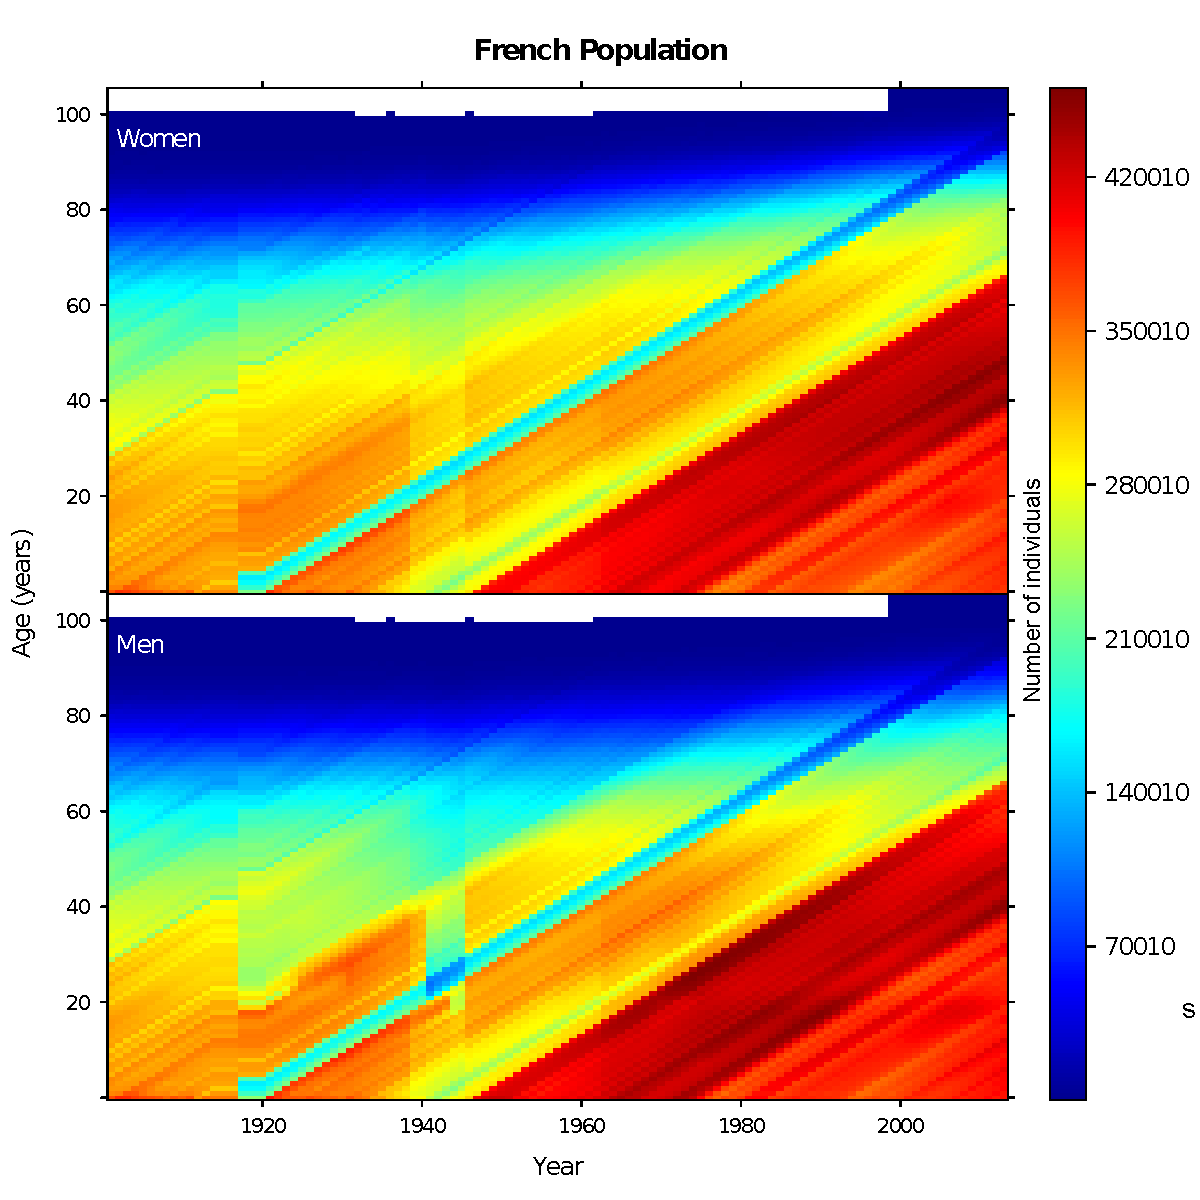
\includegraphics[width=0.9\textwidth]{2_Methodo/Fig/06}
\caption[\lofimage{2_Methodo/Fig/06}The
French age structure from 1901 to 2013]{ The
French age structure from 1901 to 2013 for women (top panel) and men (lower
 panel). These graphs reveal the secular increase of lifespan (underlined with a
 dotted line for women), the demographic scars left by the first and second
 world wars especially on adult men (dotted arrows) and on births (plain
 arrows), the baby-booms following the two armistices, the waves of immigrants
 during the post-war economic boom.
  }
\label{fig:ASTd6}
\end{figure}

\section{Conclusion}

A multi-dimensional diagram such as our structure-time diagram (Fig.
\ref{fig:ASTd2}b) is preferred to a simple time series representation (Fig.
\ref{fig:ASTd1}c, d) for several reasons: time series representation lacks the continuity of the structuring
element. Although time series plots and time series analyses are very powerful
and bring useful information on dynamics inside classes that are artificially
created, such as number of individuals or existence or not of a periodicity, the
small number of classes usually used and the representation in lines make it
very difficult to read and therefore detect and analyse any cross classes
dynamics. A three-dimensional diagram offers a unique and complete visual
display of the variations of the population structure and is thus a very
powerful tool for the description of a population and a convenient way of
guiding the analysis. Moreover, by juxtaposing several structure-time diagrams
one can add an extra dimension to the graphical display, such as the sex of the
individuals as in the lizard example (Fig. \ref{fig:ASTd4}) or any other
categorical variable (population, genotype etc.). If one uses the same axis for these diagrams, one
can in a glance compare the complex dynamics of several categories of
individuals.

The structure-time diagram does not need individuals to be identified from one
time to the other. And without any individual trajectories, changes in the
structure over time directly draw dynamics of cohorts (as in Fig.
\ref{fig:ASTd2}c).

STdiag can also be used to represent any type of data with a structuring factor
and an aggregate statistic. For instance, this method can be used to represent
the average mortality rate in each age-time class \autocites{vaupel1987a}, or
the evolution over time of the average size depending on the age, illustrating
the shrinkage of Soay sheeps \autocites{ozgul2009a}. It can also be used for
displaying data from a population model such as a physiologically structured one
\autocites{metz1986a}. It can also be applied to follow the temporal dynamic of
a human population structure coming for instance from medical survey to detect
any secular or seasonal changes for example (Fig. \ref{fig:ASTd5}).

Such diagrams fulfil the criteria for excellence in statistical graphics
\autocites{tufte1990a}: they show many numbers within a small space (high
data density) thus making coherent large data sets without distorting the data; they reveal the
data at several levels of detail, from fine structure to broad overview,
encourage the eyes to compare different pieces of data and induce the viewer to
think about the substance rather than about the method \autocites{tufte2001a}.

With the development of automatic data acquisition and prolific databases
\autocites{le-galliard2012a,mallard2012a,mallard2013a}, the use of such a
graphical display should become more common in population ecology but also in
many other fields such as human demography, epidemiology or medical surveys.

\section{Acknowledgments}

We thank the Programme interdisciplinaire du vivant Longévité et vieillissement
funded by the Centre National de la Recherche Scientifique (CNRS) and the French
Research National Agency (ANR EvoRange), reference ANR-09-PEXT-011 for
supporting this project.

We thank Guillaume Sapriel, Jean-Louis Galliard and Didier Guillemot for helping
us applying this method in the field of pharmaco-epidemiology and we are
grateful to the French Health National Insurance (CNAMTS) for providing the
antibiotic data used to construct Figure \ref{fig:ASTd5}.

\section{Supporting Information}

\subsection{Dynamics of a laboratory population of collembolan}

We studied the species Folsomia candida that is commonly used in laboratory and
is easy to breed and maintained \autocites{fountain2005a}. This
is an ametabolous parthenogenetic hexapod whose populations are composed only of females of
different size because the juveniles look like miniature adults and the adults
continue to moult and grow after reaching maturity. The individuals were bred at
$21\degres C$ in cylindric plastic boxes of 5.3 cm diameter with a 3 cm thick
plaster substrate to keep the environment damp \autocites[Fig.
\ref{fig:ASTd1}]{tully2008a}. The population is fed weekly with a mix of
yeast in agar-agar in a fixed quantity and kept in the dark the whole time.

\subsection{Dynamics of a wild population of common lizards}

The studied population comes from the Mont Lozère in southern France (1420 m
a.s.l, $44\degres 30’N, 3 \degres 45’E$). Data collection each year was
structured as follows:
a capture session of yearlings (1 year old individuals) and adults in June-July
and a temporary transfer of pregnant females to the laboratory to mark and
measure juveniles from birth \autocites{le-galliard2010a}.
We used a total of 7486 measurements, 3935 females and 3551 males.

\subsection{Code for generating the plots in Figure \ref{fig:ASTd2}}

Here is the code for generating the Figure \ref{fig:ASTd2}. We used the data
“sample” which is provided in the library STdiag.
\begin{verbatim}
data(sample)
st1=STdiag(z~x*y,data=sample,xlab="Time",ylab="Structure",color="gray",main="Gray Palette")
st2=STdiag(z~x*y,data=sample,xlab="Time",ylab="Structure",color="tim",main="Tim Palette")
st3=STdiag(z~x*y,data=sample,xlab="Time",ylab="Structure",color="tim",
    main="Log Color Scale",log=T)
st4=STdiag(z~x*y,data=Interpolation(sample),xlab="Time",ylab="Structure",
    color="tim",main="Interpolated data",log=T)
st5=STdiag(z~x*y,data=Interpolation(sample),xlab="Time",ylab="Structure",
    color="tim",main="sm = 0.2",log=T,smooth=T,sm=0.2)
st6=STdiag(z~x*y,data=Interpolation(sample),xlab="Time",ylab="Structure",
    color="tim",main="sm = 0.6",log=T,smooth=T,sm=0.6)
pdf(file="figSTdiag.pdf",width=7, height=16*7/9)
print(st1) ; print(st2) ; print(st3) ; print(st4) ; print(st5) ; print(st6)
dev.off()
\end{verbatim}